\chapter{Ultrasound}
\vspace{-40ex}\hspace{35ex}
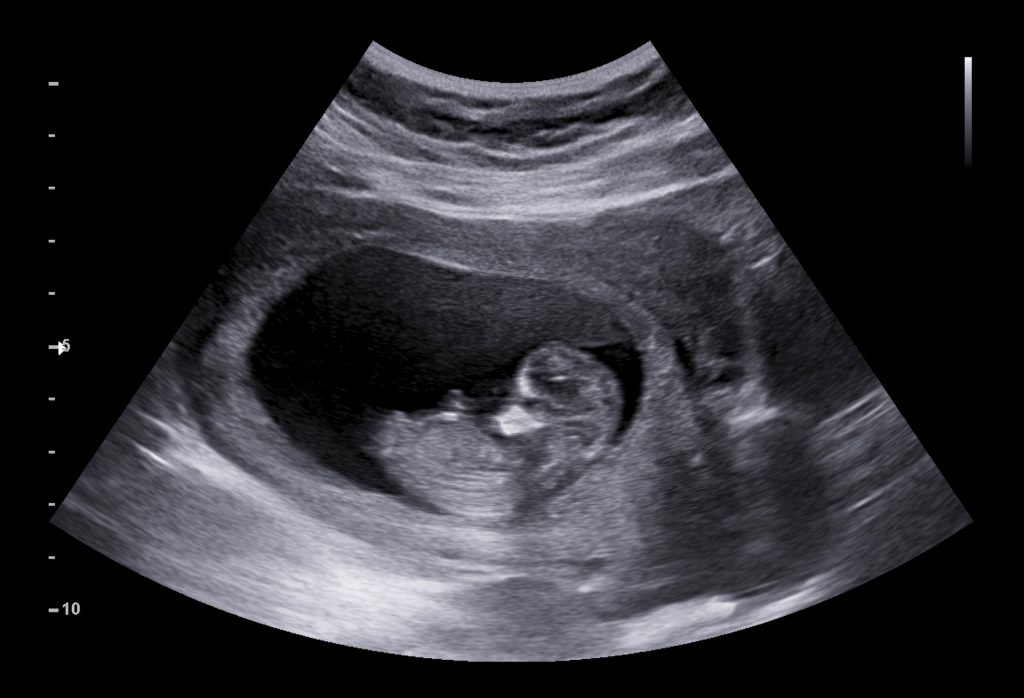
\includegraphics[width=10cm]{fetus_2D}

\section{Properties of sound}

\begin{itemize}
\item Mechanical energy in the form of \popup{high-frequency}{The
    higher the frequency the better resolution and image detail, but
    lower penetration.} (usually in the range of 2 to 18 MHz
  \cite{abdulla2025sound}) \popup{sound waves}{Sound waves are
    longitudinal preasure mechanical waves. They need a medium to
    propagate at a speed that depends on the rigidity and density of
    the medium. The typical speed in the tissue is 1540 m/s.} can be
  used to generate images of the anatomy of a patient (see Figure
  \ref{fig:sound}).
\end{itemize}
%\vspace{-2ex}
\begin{figure}[!h]
  \centering
  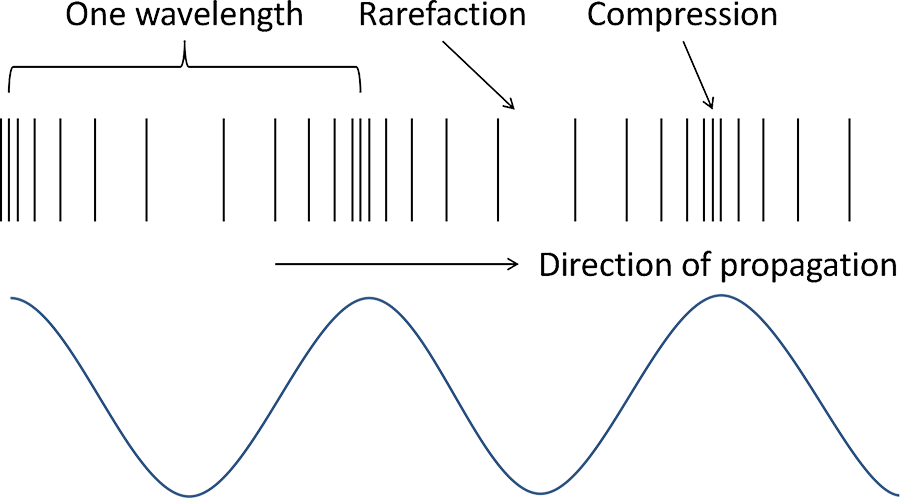
\includegraphics[width=8cm]{sound}
  \caption{Mechanical movement of the particles with the sound
    \cite{abdulla2025properties_sound}.\label{fig:sound}}
\end{figure}

\section{Echoes}
\begin{itemize}
\item \popup{(Ultra)Sound waves}{In form of decaying pulses.} pass
  through tissues, get reflected, and the returning wave (echo) is
  detected and forms the
  image\cite{bushberg2011essential,abdulla2025ultrasound_machine}. In
  \popup{B-mode}{B for Brightness (the most common ultrasound imaging
    used in medicine). There is A-Mode (A for Amplitude) that is
    mainly used in ophthalmology to investigate retinal detachment.}
  imaging, the intensity of the returning wave (echo) is represented
  as a level of brightness on the monitor to give a 2D cross-sectional
  image on the monitor \cite{abdulla2025ultrasound} (see Figure
  \ref{fig:interactions}).
\end{itemize}
%\vspace{-3ex}
\begin{figure}[!h]
  \centering
  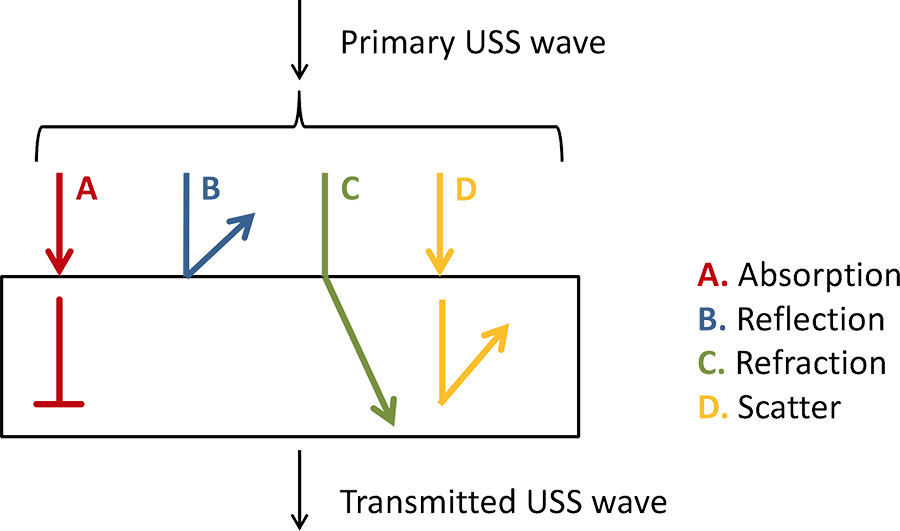
\includegraphics[width=7cm]{sound_interactions}
  \caption{Interactions of the ultrasound scan (USS) with tissue
    \cite{abdulla2025properties_sound}.\label{fig:interactions}}
\end{figure}

\section{Ultrasound imaging with flow detection}
\begin{itemize}
\item It is possible to use the \popup{M-Mode}{M for Motion.} (based
  on the Doppler effect) to detect the motion of fluids and mobile
  structures
  \cite{bushberg2011essential,abdulla2025ultrasound_machine}. Thus,
  for example, we can \popup{measure the blood flow}{Both the speed
    and direction of blood flow can be measured, and within a subarea
    of the grayscale image, a color flow display typically shows blood
    flow in one direction as red, and in the other direction as
    blue.}, displayed as color channels \cite{bushberg2011essential}
  (see Figure~\ref{fig:doppler}).
\end{itemize}
%\vspace{-4ex}
\begin{figure}[!h]
  \centering
  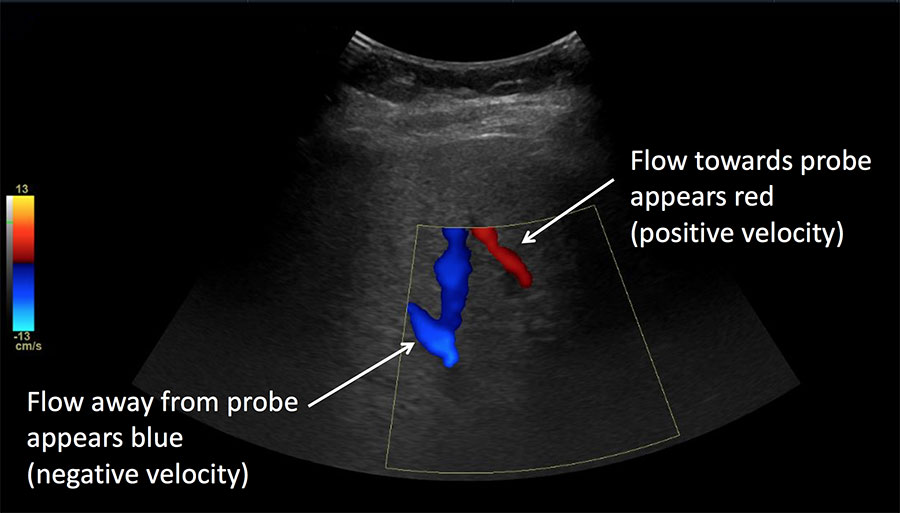
\includegraphics[width=8.0cm]{doppler}
  \caption{Ultrasound image showing flood motion
    \cite{abdulla2025ultrasound_imaging_doppler}.\label{fig:doppler}}
\end{figure}

\section{3D rendering}
\begin{itemize}
\item Ultrasound imaging is basically a \popup{2D technique}{By
    default, an ultrasound machine shows a deformed slice of the
    structure to analyze.}. However, 3D images can be generated by
  placing the known voxels in a
  \href{https://stackoverflow.com/questions/51907238/how-to-draw-a-2d-3d-grid-from-buffergeometry-in-three-js}{3D
    grid},
  \href{https://en.wikipedia.org/wiki/Trilinear_interpolation}{interpolating}
  the unknown voxels, and then,
  \href{https://en.wikipedia.org/wiki/Image_segmentation}{segmenting}
  (see Figure~\ref{fig:fetus_3D}).
\end{itemize}
%\vspace{-4ex}
\begin{figure}[!h]
  \centering
  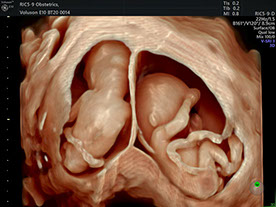
\includegraphics[width=6.0cm]{fetus_3D}
  \caption{3D ultrasound reconstruction
    \cite{fetal_diagnostic_centers}.\label{fig:fetus_3D}}
\end{figure}

\section{Artifacts}
\begin{itemize}
\item Image formation assumes that sound travels in straight lines, at
  a constant velocity, with uniform attenuation, and reflected only
  once from each interface \cite{abdulla2025ultrasound_artefacts}.
\item \popup{Artefacts}{Or artifacts, depending where you live!}
  result when the echo does not behave in this way and the system
  misinterprets it.
\end{itemize}

\section*{}
\subsection{Enhancement}
\begin{itemize}
\item Fluid filled structures are weakly
  \popup{attenuated}{Consequently, a larger proportion and greater
    amplitude beam passes through to structures in the region behind},
  and the image reconstruction algorithm interprets this as an
  \popup{increase in acoustic reflection}{The structures below show up
    brighter on the image.} (see
  Figure~\ref{fig:acoustic_enhancement}).
\end{itemize}
%\vspace{-3ex}
\begin{figure}[!h]
  \centering
  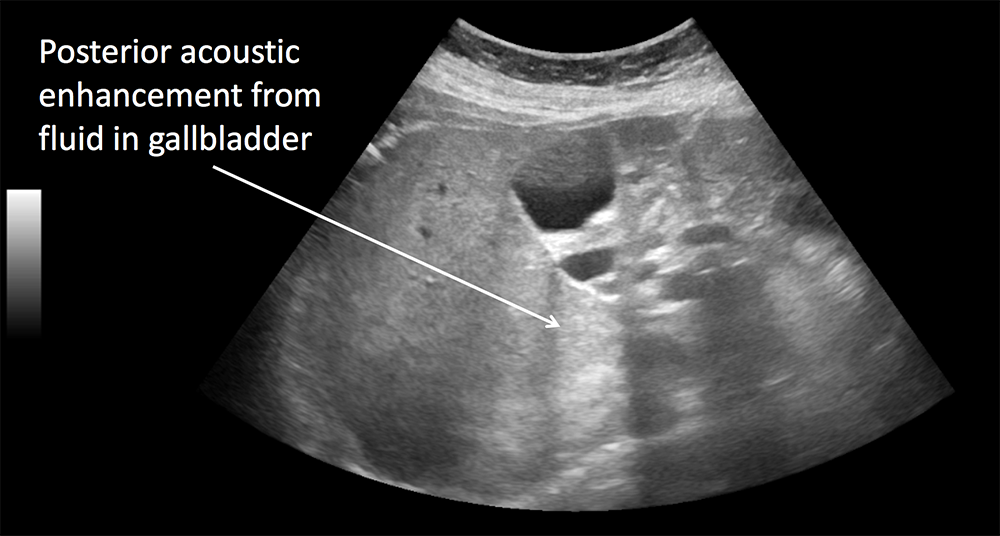
\includegraphics[width=8cm]{acoustic_enhancement}
  \caption{Acoustic enhancement artefact in ultrasound
    \cite{abdulla2025ultrasound_artefacts}.\label{fig:acoustic_enhancement}}
\end{figure}

\section*{}
\subsection{Shadowing}
\begin{itemize}
\item Hard calcific substances and soft tissue-air interfaces reflect almost all of the soundwaves. Therefore, no information is received from the area behind the structure (see
  Figure~\ref{fig:acoustic_shadowing}).
\end{itemize}
\vspace{-1ex}
\begin{figure}[!h]
  \centering
  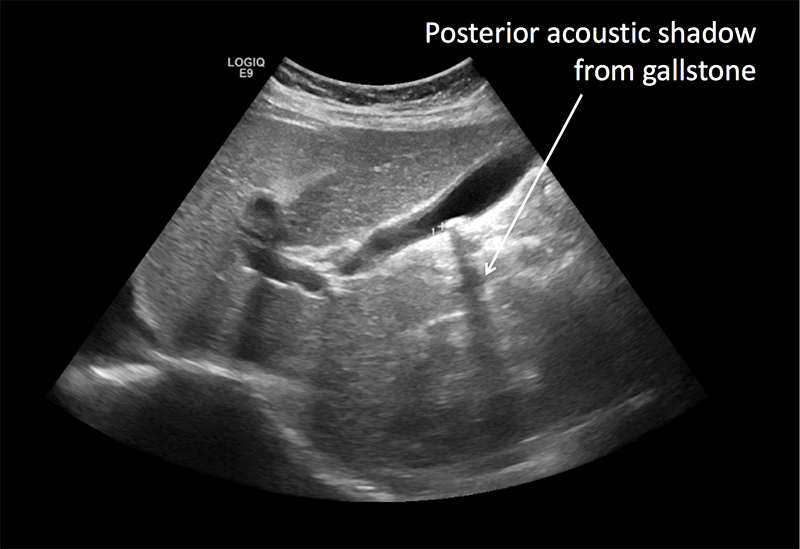
\includegraphics[width=6.5cm]{acoustic_shadowing}
  \caption{Acoustic shadowing artefact in ultrasound
    \cite{abdulla2025ultrasound_artefacts}.\label{fig:acoustic_shadowing}}
\end{figure}

\section*{}
\subsection{Reverberation}
\begin{itemize}
\item Reverberation artifacts occur when sound waves bounce back and
  forth between two surfaces, creating \popup{multiple echoes}{These
    echoes appear as parallel lines on the image, giving the
    appearance of multiple objects or structures.}. (see
  Figure~\ref{fig:acoustic_reverberation}) \cite{NysoraArtifacts}.
\end{itemize}
\vspace{-1ex}
\begin{figure}[!h]
  \centering
  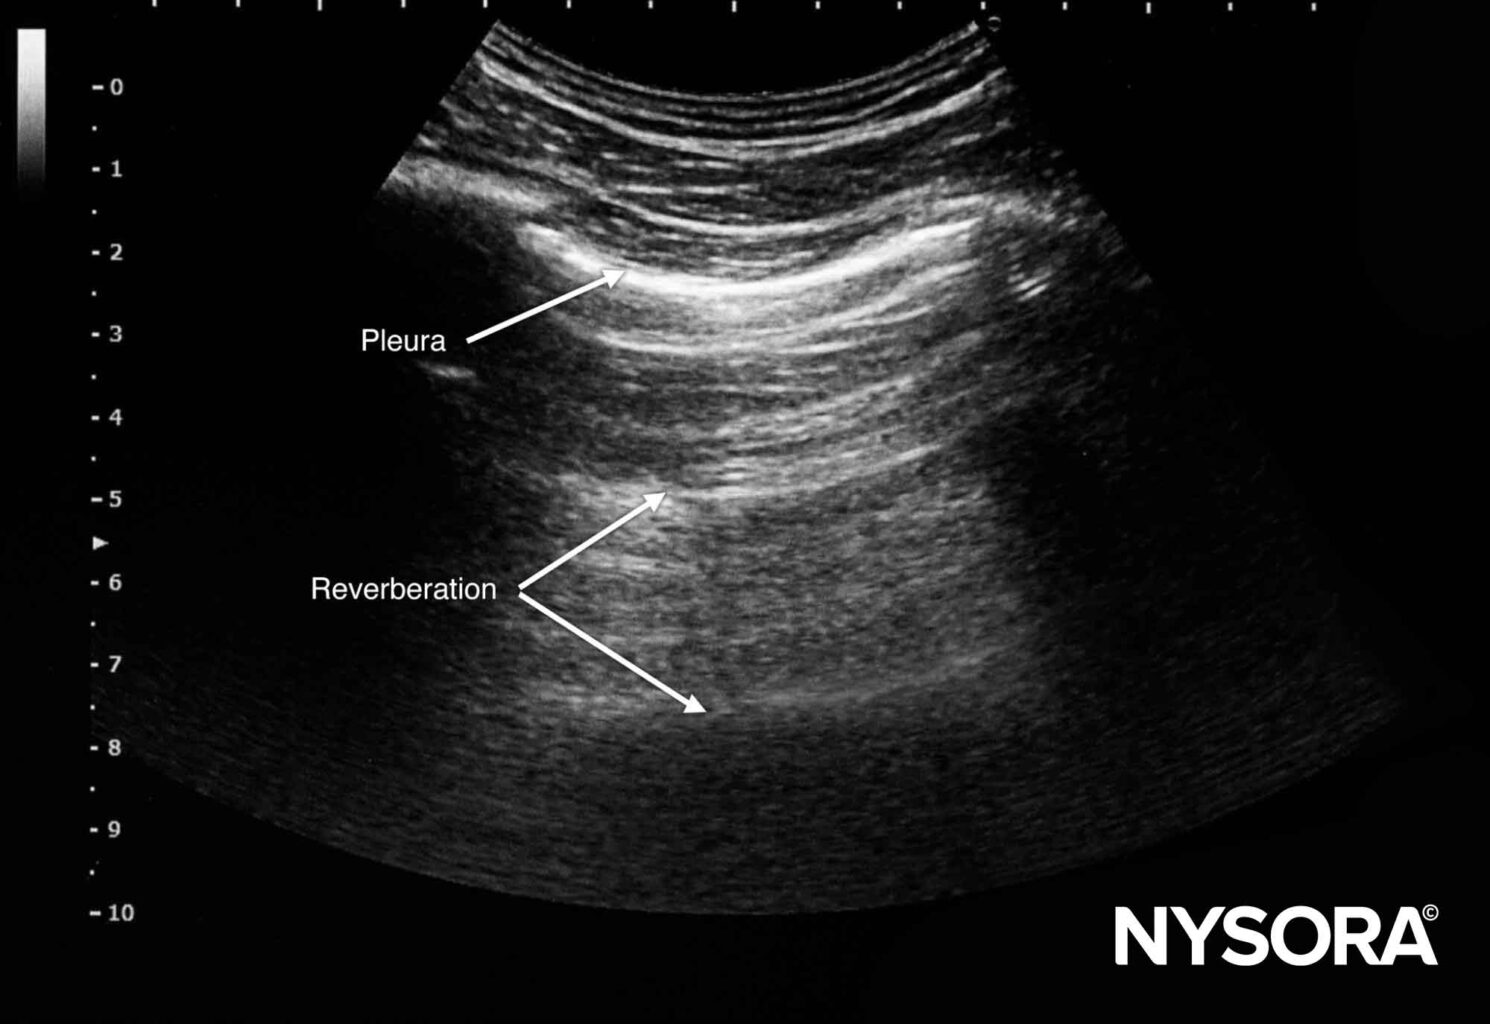
\includegraphics[width=6.5cm]{acoustic_reverberation}
  \caption{Acoustic reverberation artefact in ultrasound
    \cite{NysoraArtifacts}.\label{fig:acoustic_reverberation}}
\end{figure}

\section*{}
\subsection{Speckle}
\begin{itemize}
\item \popup{Speckle artifacts}{Also known by speckle noise.} are
  caused by the interference of sound waves with the echoes, resulting
  in a granular or \popup{speckled appearance of the image}{These
    artifacts can make it difficult to distinguish between small
    structures, such as blood vessels.}  \cite{NysoraArtifacts} (see
  Figure~\ref{fig:acoustic_speckle}).
\end{itemize}
\vspace{-2ex}
\begin{figure}[!h]
  \centering
  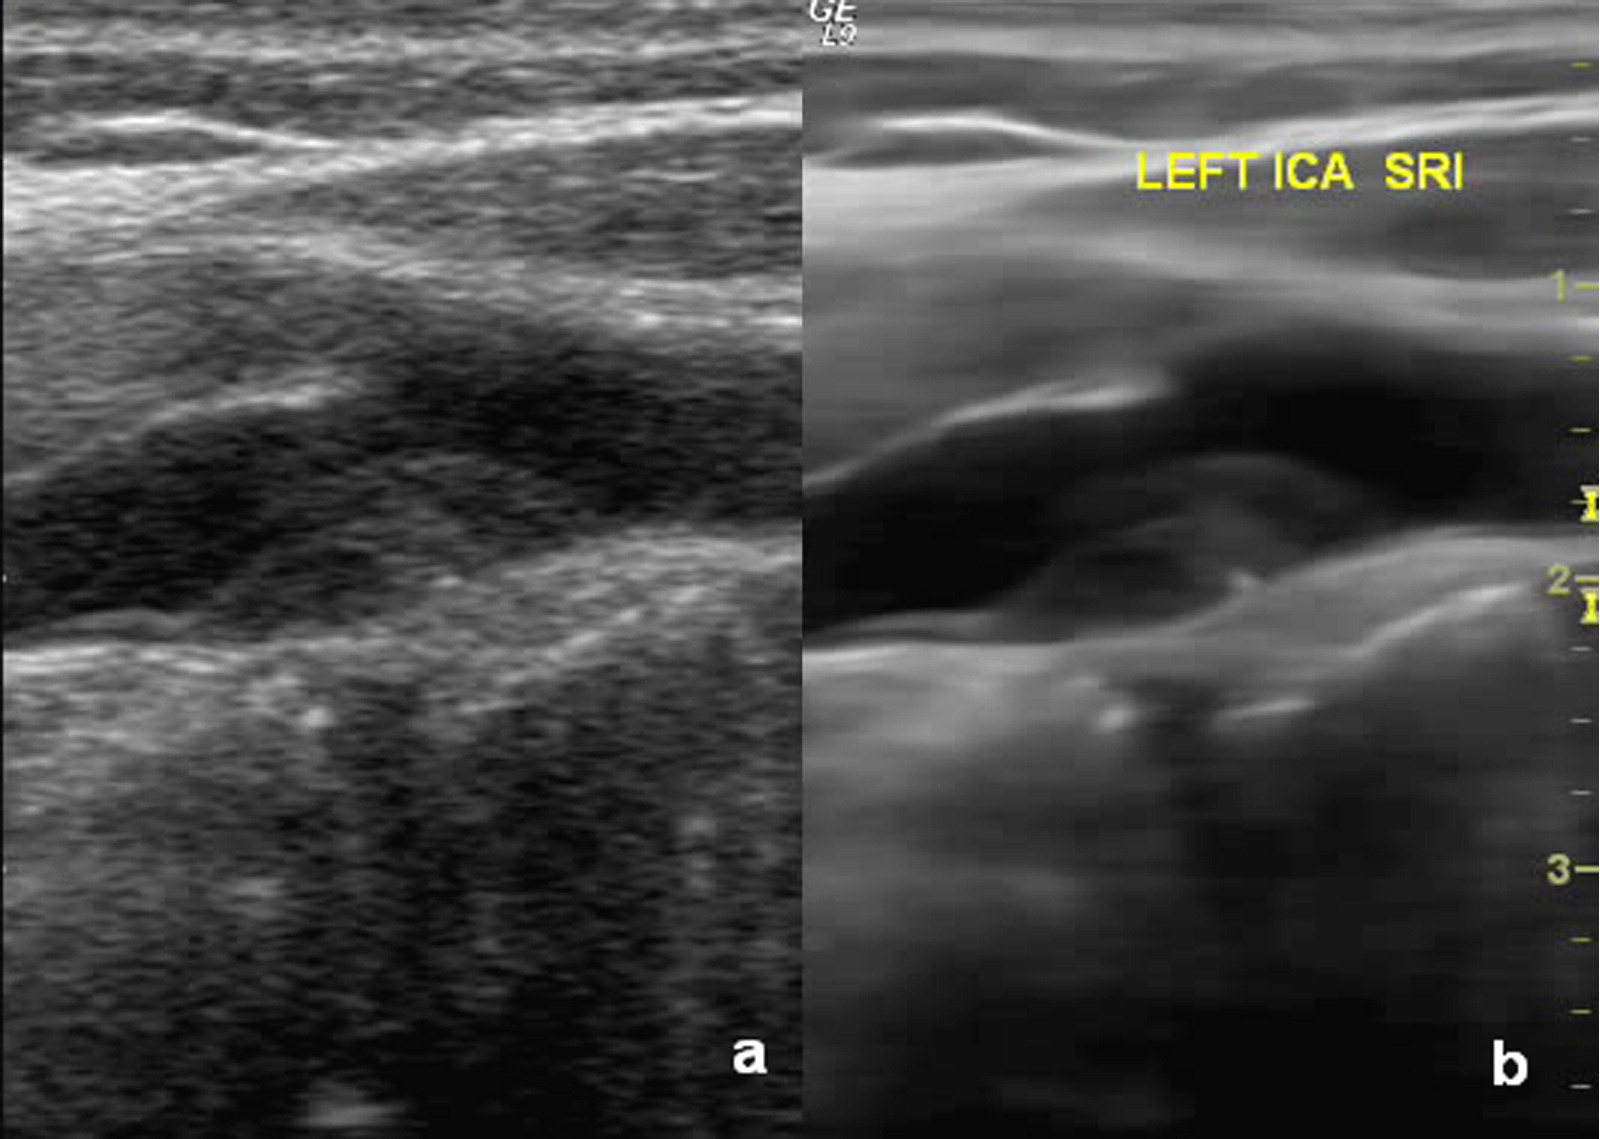
\includegraphics[width=6.5cm]{acoustic_speckle}
  \caption{Speckle noise in ultrasound
    \cite{LIASIS2008427}.\label{fig:acoustic_speckle}}
\end{figure}

\section*{}
\begin{itemize}
\item Speckle is usually modeled as \popup{multiplicative
    noise}{Multiplicative noise is proportional to the intensity of
    the clean signal.}. Its amplitude (which depends on the clean
  signal) follows a
  \href{https://en.wikipedia.org/wiki/Rayleigh_distribution}{Rayleigh
    distribution}, and its phase is
  \href{https://en.wikipedia.org/wiki/Discrete_uniform_distribution}{uniformly
    distributed}.

\item If multiple images are taken (changing the angle and
  orientation) and averaged \emph{spatial compounding}, speckle noise
  dimishes following a
  \href{https://en.wikipedia.org/wiki/Gamma_distribution}{Gamma
    distribution} \cite{bushberg2011essential}.
\end{itemize}
